\documentclass[a4paper]{article}

\usepackage{amsmath}
\usepackage{amssymb}
\usepackage{stellar}
\usepackage{parskip}
\usepackage{fullpage}
\usepackage{tikz}

\usetikzlibrary{arrows}
\usetikzlibrary{decorations.pathreplacing}

\title{Precorso}
\author{Paolo Bettelini}
\date{}

% algebrainsubria.altervista.org

\begin{document}

\maketitle
\tableofcontents

\pagebreak

\section{Connettori logici}

\sdefinition{Proposizione}{
    Una \textit{proposizione} è un'espressione che può essere \text{vera} o \text{falsa}.
}

\sdefinition{Connettore logico e}{
    Date due proposizioni \(P\) e \(Q\), \(P \land Q\), è un'altra
    proposizione vera solamente se \(P\) è vera e \(Q\) è vera.
}

\begin{center}
    \begin{tabular}{|c|c|c|}
        \hline
        \(\land\) & \text{falso} & \text{vero} \\
        \hline
        \text{falso} & \text{falso} & \text{falso} \\
        \hline
        \text{falso} & \text{vero} & \text{falso} \\
        \hline
        \text{vero} & \text{falso} & \text{falso} \\
        \hline
        \text{vero} & \text{vero} & \text{vero} \\
        \hline
    \end{tabular}    
\end{center}

\sdefinition{Connettore logico oppure}{
    Date due proposizioni \(P\) e \(Q\), \(P \lor Q\), è un'altra
    proposizione vera se \(P\) è vera oppure \(Q\) è vera (o entrambe sono vere).
}

\begin{center}
    \begin{tabular}{|c|c|c|}
        \hline
        \(\lor\) & \text{falso} & \text{vero} \\
        \hline
        \text{falso} & \text{falso} & \text{falso} \\
        \hline
        \text{falso} & \text{vero} & \text{vero} \\
        \hline
        \text{vero} & \text{falso} & \text{vero} \\
        \hline
        \text{vero} & \text{vero} & \text{vero} \\
        \hline
    \end{tabular}    
\end{center}

\section{Teoria ingenua degli insiemi}

\sdefinition{Insieme ingenuo}{
    Un \textit{insieme} è una collezione di oggetti di qualunque tipo,
    detti \textit{elementi dell'insieme}.
    Diciamo che un elemento \(a\) appartiene ad un insieme \(A\) con \(a \in A\),
    mentre \(a \notin A\) se non appartiene.
}

\sexample{Insieme}{
    \[ A = \{3, 5, -3, \sqrt{5}, \phi \} \]
    dove \(\phi\) è una funzione.
}

È importante notare che l'ordine degli elementi non ha importanza.
Un insieme può contenere tra i suoi elementi anche altri insiemi.

Un insieme viene spesso descritto per mezzo di una proprietà comune dei suoi elementi,
piuttosto che per elencazione estensiva.

\sexample{Insieme costruito per proprietà}{
    \[ D = \{ n \,|\, n = m^2 -1, \quad m \in \mathbb{N} \} \]
}

In generale, può essere difficile determinare se un elemento appartiene ad un certo insieme o meno.
Per esempio, non è sempre facile determinanre se un grande numero appartiene all'insieme di tutit i
numeri primi. In alcuni casi, è difficile addirittura stabilire se un insieme contenga elementi, o quanti
ne contenga. Tuttavia, questo difficoltà non implica che l'insieme non sia ben definito.

%\sdefinition{Cardinalità}{
%    La \textit{cardinalità} di un insieme \(A\), detta \(|A|\),
%    ha valore pari al numeri di elementi contenenti in \(A\).
%}

\sdefinition{Sottoinsieme}{
    Dati due insiemi \(A\) e \(B\), diciamo che \(A\) è un \textit{sottoinsieme} di \(B\),
    se ogni elemento di \(A\) è un elemento di \(B\).
    \[ A \subseteq B \iff B \supseteq A \iff \forall a \in A, a\in B \]
    In caso contrario, diciamo che \(A \not\subseteq B\) oppure \(B \not\supseteq A\)
}

\sexample{Sottoinsieme}{
    \[ \{ 1, 3, 5, 7, 11 \} \subseteq \{ \text{ insieme dei numeri dispari } \} \]
    \[ \{ 1, 3, 5, 8, 11 \} \not\subseteq \{ \text{ insieme dei numeri dispari } \} \]
}

\sdefinition{Sottoinsieme proprio o stretto}{
    Dati due insiemi \(A\) e \(B\), diciamo che \(A\) è un \textit{sottoinsieme proprio } di \(B\),
    se ogni elemento di \(A\) è un elemento di \(B\) ma \(A \neq B\).
    \[ A \subset B \iff B \supset A \iff \forall a \in A, a\in B \land A \neq B \]
    In caso contrario, diciamo che \(A \not\subset B\) oppure \(B \not\supset A\)
}

\sexample{Sottoinsieme proprio}{
    \[ \{ 1, 3, 5 \} \subset \{ 1, 3, 4, 5 \} \]
}

Alcuni insiemi convenzionali sono:
\begin{itemize}
    \item \textbf{Insieme dei numeri naturali:} \(\mathbb{N} = \{0,1,2,\cdots\}\);
    \item \textbf{Insieme dei numeri interi:} \(\mathbb{Z} = \{\cdots, -2, -1, 0,1,2,\cdots\}\);
    \item \textbf{Insieme dei numeri razionali:} \(\mathbb{Q} = \{ \frac{m}{n} \,|\, m,n \in \mathbb{Z} \land n \neq 0 \}\);
    \item \textbf{Insieme dei numeri reali:} \(\mathbb{R}\);
    \item \textbf{Insieme dei numeri complessi:} \(\mathbb{C} = \{a + bi \,|\, a,b \in \mathbb{R}\}\);
\end{itemize}

\subsection{Operazioni tra insiemi}

\sdefinition{Intersezione}{
    Dati degli insiemi \(A\) e \(B\), l'\textit{intersezione} di \(A\) e \(B\) è data da
    gli insiemi che stanno sia in \(A\) che in \(B\)
    \[ A \cap B = \{ x \,|\, x \in A \land b \in B\} \]
}

\sdefinition{Unione}{
    Dati degli insiemi \(A\) e \(B\), l'\textit{unione} di \(A\) e \(B\) è data da
    gli insiemi che stanno o in \(A\) o in \(B\)
    \[ A \cup B = \{ x \,|\, x \in A \lor b \in B\} \]
}

\sdefinition{Differenza}{
    Dati degli insiemi \(A\) e \(B\), la \textit{differenza} di \(A\) e \(B\) è data da
    gli insiemi che stanno in \(A\) ma non in \(B\)
    \[ A \,\backslash\, B = \{ x \,|\, x \in A \land b \notin B\} \]
}

\sexample{Intersezione}{
    \[
        \{ 1,3,5,7,9,11 \} \,\backslash\, \{ \text{ insieme dei numeri primi } \}
        = \{ 1,9 \}
    \] \[
        \{ \text{ insieme dei numeri primi } \} \,\backslash\, \{ 1,3,5,7,9,11 \}
        = \{ \text{ insieme dei numeri primi } > 13 \}
    \]
}

Nota che, convenzionalmente, nella definizione dei numeri primi il numero \(1\) è escluso.

\begin{center}
    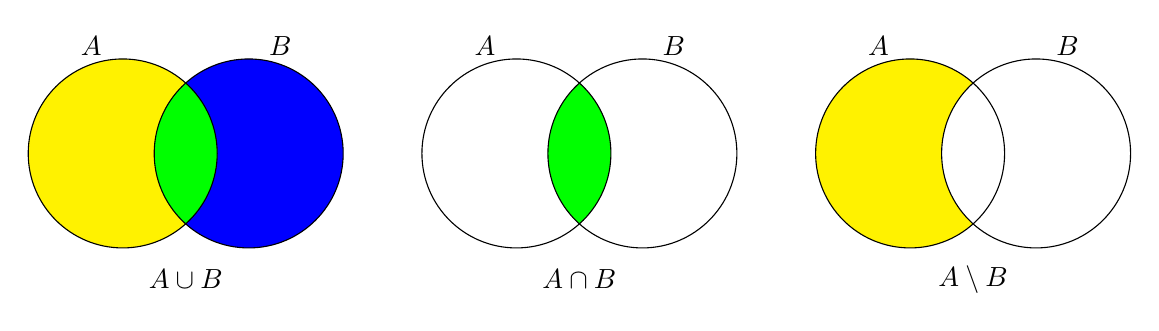
\begin{tikzpicture}
        % Union A ∪ B
        \begin{scope}[shift={(-5,0)}, scale=0.8]
            \fill[yellow] (-1,0) circle (1.5);
            \fill[blue] (1,0) circle (1.5);
            \begin{scope}
                \clip (-1,0) circle (1.5);
                \fill[green] (1,0) circle (1.5);
            \end{scope}
            \draw (-1,0) circle (1.5);
            \draw (1,0) circle (1.5);
            \node at (-1.5, 1.7) {$A$};
            \node at (1.5, 1.7) {$B$};
            \node at (0, -2) {$A \cup B$};
        \end{scope}
    
        % Intersection A ∩ B (only middle part)
        \begin{scope}[shift={(0,0)}, scale=0.8]
            \fill[white] (-1,0) circle (1.5);
            \fill[white] (1,0) circle (1.5);
            \begin{scope}
                \clip (-1,0) circle (1.5);
                \fill[green] (1,0) circle (1.5);
            \end{scope}
            \draw (-1,0) circle (1.5);
            \draw (1,0) circle (1.5);
            \node at (-1.5, 1.7) {$A$};
            \node at (1.5, 1.7) {$B$};
            \node at (0, -2) {$A \cap B$};
        \end{scope}
    
        % Difference A \ B (same as before)
        \begin{scope}[shift={(5,0)}, scale=0.8]
            \fill[yellow] (-1,0) circle (1.5);
            \fill[white] (1,0) circle (1.5);
            \begin{scope}
                \clip (1,0) circle (1.5);
                \fill[white] (-1,0) circle (1.5);
            \end{scope}
            \draw (-1,0) circle (1.5);
            \draw (1,0) circle (1.5);
            \node at (-1.5, 1.7) {$A$};
            \node at (1.5, 1.7) {$B$};
            \node at (0, -2) {$A \setminus B$};
        \end{scope}
    \end{tikzpicture}
\end{center}

Il disegno suggerisce la seguente proposizione 
\sproposition{}{
    Dati due insiemi \(A\) e \(B\)
    \[
        A = (A \,\backslash\, B) \cup (A \cap B)
    \]
}

Si può dimostrare separatamente che ogni elemento del primo insieme appartiene al secondo e viceversa.
Prendiamo quindi \(x\in A\), bisogna mostrare che
\(x \in A \,\backslash\, B\) oppure \(x \in A \cap B\), siccome si tratta di una intersezione fra due insiemi.
Abbiamo quindi che almeno una delle seguenti proposizioni deve essere vera:
\begin{enumerate}
    \item \(x \in A \land x \notin B\)
    \item \(x \in A \land x \in B\)
\end{enumerate}

Se \(x \in B\), allora \(x \in A \cap B\).
Se \(x \notin B\), allora \(x \in A \,\backslash\, B\)
Di conseguenza, almeno una delle due è vera.

Viceversa, sia \(x \in (A \,\backslash B) \cup (A \cap B)\).
Abbimo quindi che almeno una delle seguenti proposizioni è vera
\begin{enumerate}
    \item \(x \in A \land x \notin B\) quind \(x \in A \,\backslash B\)
    \item \(x \in A \land x \in B\) quindi \(x \in A \cap B\)
\end{enumerate}
Se la prima è vera, entrambi \(x \in A\) e \(x \notin B\) sono vere (in particolare, \(x \in A\) è vera).
Se la seconda è vera, entrambe \(x\in A\) e \(x \in B\) sono vere (in particolare, \(x \in A\) è vera).
In ogni caso, \(x \in A\) è vera.

\pagebreak

\subsection{Proprietà delle operazioni fra insiemi}

\sproposition{}{
    Dati tre insiemi \(A\), \(B\) e \(C\)
    \begin{itemize}
        \item \textbf{Intersezione commutativa:} \(A \cap B = B \cap A\)
        \item \textbf{Unione commutativa:} \(A \cup B = B \cup A\)
        \item \textbf{Intersezione associative:} \((A \cap B) \cap C = A \cap (B \cap C)\)
        \item \textbf{Unione associative:} \((A \cup B) \cap C = A \cup (B \cup C)\)
        \item \textbf{Distributiva:} \(A \cap (B \cup C) = (A \cap B) \cup (A \cap C)\)
        \item \textbf{Distributiva:} \(A \cup (B \cap C) = (A \cup B) \cap (A \cup C)\)
    \end{itemize}
}

Di conseguenza, \(A \cap B \cap C\) e \(A \cup B \cup C\) non sono ambigue.

Data una famiglia di insiemi \({\{A_i\}}_{i \in I}\) dove \(I\) è un insieme di indici,
è possibile eseguire l'unione e intersezioni
\[
    \bigcup_{i\in I} A_i
\]
e
\[
    \bigcap_{i\in I} A_i
\]
ossia rispettivamente l'insieme che contiene tutti gli elementi di tutti gli insiemi \(A_i\) e quello
che tutti gli insiemi \(A_i\) hanno in comune.

\sproposition{}{
    Dati due insiemi \(A\) e \(B\)
    \[ (A \,\backslash\, B) \cap (B \,\backslash\, A) = \emptyset \]
}

Chiaramente, nessun elemento soddisfa la condizione data,
in quando un elemento dovrebbe sia appartenente ad \(A\) e non appartenente ad \(A\), e
sia appartenente a \(B\) che non appartenente a \(B\).

\sdefinition{Prodotto cartesiano}{
    Dati due insiemi \(A\) e \(B\), il loro \textit{prodotto cartesiano} è dato dall'insieme delle coppie ordinate
    \[ A \times B = \{ (a,b) \,|\, a\in A \land b\in B \} \]
}

\sexample{Prodotto cartesiano}{
    Dati \(A = \{0,1,2\}\) e \(B=\{1,2,3\}\) abbiamo
    \[
        A \times B = \{
            (0,1),
            (0,2),
            (0,3),
            (1,1),
            (1,2),
            (1,3),
            (2,1),
            (2,2),
            (2,3)    
        \}
    \]
}

Questa operazione non è commutativa, in quando le coppie ordinate di \(A \times B\)
e \(B \times A\) hanno le coppie di elementi scambiate.

\sdefinition{Prodotto cartesiano generalizzato}{
    Dati degli insiemi \(A_1\), \(A_2\), \(\cdots\), \(A_n\),
    il loro \textit{prodotto cartesiano} è dato dall'insieme delle n-uple
    \[
        A_1 \times A_2 \times \cdots \times A_n =
        \{ (a_1, a_2, \cdots, a_n) \,|\, a_1 \in A_1 \land a_2 \in A_2 \cdots a_n \in A_n \}
    \]
}

Chiaramente, per ogni insieme \(A\), \(A \times \emptyset = \emptyset\)

\subsection{Corrispondenze e funzioni}

\sdefinition{Corrispondenza}{
    Dati due insiemi \(A\) e \(B\), una \textit{corrispondenza} \(\sim\) 
    fra \(A\) e \(B\) è una legge che lega gli elementi di \(A\) e \(B\)
    \[ \sim\, \subseteq A \times B \]
    Diciamo che \(a\in A\) è in relazione con \(b \in B\) se la tupla
    \((a,b)\) è in \(\sim\).
}

\sdefinition{Operatore divisione}{
    Dati \(m,n\in\mathbb{N}\), possiamo mettere in relazione \(m\) e \(n\), dicendo che \(m\)
    divide \(n\), scrivendo \(m \,|\, n\).
}

La divisione fra interi induce una corrispondenza \(\sim\, \subseteq {\mathbb{N}}^2\)
dove \(x \sim y \iff x \,|\, y\).
Alcuni elementi di questa corrispondenza sono \((1,2), (1,100), (2, 50), (50, 250)\).
Possiamo anche scrivere \(50 \sim 250\) oppure \(50 \not\sim 251\).

\sdefinition{Funzione}{
    Dati due insiemi \(A\) e \(B\), una \textit{funzione} \(\phi\) da \(A\) a \(B\),
    scritta \(\phi\colon A \to B\)
    è una corrispondenza da \(A\) a \(B\) in cui per ogni tupla \((a,b)\), non vi sono
    altre tuple \((a,c)\) dove \(c\neq a\), e per ogni \(a\in A\) vi è una corrispondenza \((a,b)\).
    \[
        \phi \subset A \times B
    \]
    L'insieme \(A\) è detto \textit{domanio}, mentre l'insieme \(B\) è detto \textit{codominio}.
}

\begin{center}
    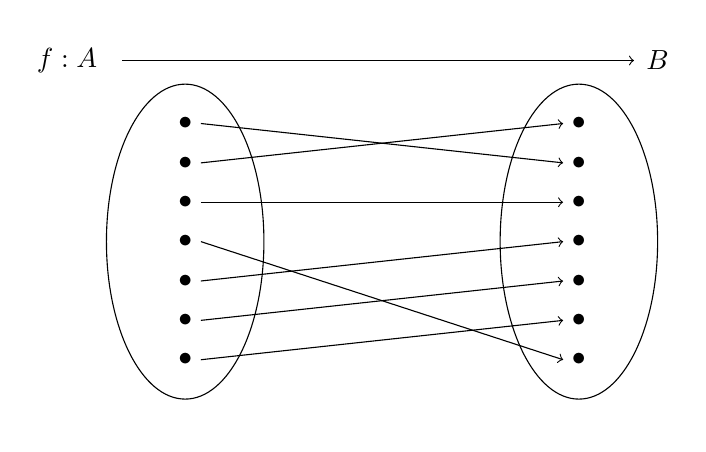
\begin{tikzpicture}
        %sets A and B
        \draw (0,0) ellipse (1 and 2);
        \draw (5,0) ellipse (1 and 2);
        \node at (-1.5,2.3) {$f:A$};
        \node at (6,2.3) {$B$};
        \draw[->] (-0.8,2.3) -- (5.7,2.3);
        
        %set A
        \node at (0,-1.5) {$\bullet$};
        \node at (0,-1) {$\bullet$};
        \node at (0,-0.5) {$\bullet$};
        \node at (0,0) {$\bullet$};
        \node at (0,0.5) {$\bullet$};
        \node at (0,1) {$\bullet$};
        \node at (0,1.5) {$\bullet$};
        
        %set B
        \node at (5,-1.5) {$\bullet$};
        \node at (5,-1) {$\bullet$};
        \node at (5,-0.5) {$\bullet$};
        \node at (5,0) {$\bullet$};
        \node at (5,0.5) {$\bullet$};
        \node at (5,1) {$\bullet$};
        \node at (5,1.5) {$\bullet$};
        
        %arrows
        \draw[->] (0.2,-1.5) -- (4.8,-1);
        \draw[->] (0.2,-1) -- (4.8,-0.5);
        \draw[->] (0.2,-0.5) -- (4.8,0);
        \draw[->] (0.2,0) -- (4.8,-1.5);
        \draw[->] (0.2,0.5) -- (4.8,0.5);
        \draw[->] (0.2,1) -- (4.8,1.5);
        \draw[->] (0.2,1.5) -- (4.8,1);
    
        %spacer
        \node at (0,2.6) {\phantom{}};
        \node at (0,-2.2) {\phantom{}};
    \end{tikzpicture}
\end{center}

Ogni funzione deve avere una (sola) freccia che parte da ogni punto.


In parole povere ciò significa che una funziona deve associare ogni elemento di \(A\) ad un elemento di
\(B\), ma solo ed unicamente uno. Elementi di \(A\) diversi possono essere in relazione con lo stesso elemento di \(B\).

\sexample{Funzione}{
    La corrispondenza da \(A=\mathbb{Z}\) a \(B=\mathbb{Z}\)
    data da \(a \sim b \iff b^2 = a\) è una funzione.
    \[
        \phi\colon \mathbb{Z} \to \mathbb{Z}
    \]
    La corrispondenza opposta \(a \sim b \iff a^2 = b\) non è una funzione perché non tutti gli elementi hanno
    una corrispondenza.
}

\pagebreak

\sexample{Funzione}{
    La corrispondenza da \(A=\mathbb{R}\) a \(B={\mathbb{R}}^+\)
    data da \(a \sim b \iff a = b^2\) è una funzione, ma non l'inverso.
    \[
        \phi\colon \mathbb{R} \to {\mathbb{R}}^+
    \]
}

\sexample{Funzione}{
    La corrispondenza da \(A={\mathbb{R}}^+\) a \(B={\mathbb{R}}^+\)
    data da \(a \sim b \iff a = b^2\) è una funzione, e pure il suo inverso
    da \(B\) ad \(A\).
    \[
        \phi\colon {\mathbb{R}}^+ \to {\mathbb{R}}^+
    \]
}

\sdefinition{Funzione identica}{
    Dato un insieme \(A\), una funzione 
    \[
        \phi\colon A\to A
    \]
    è detta \textit{identica} \(I_A\), se ogni elemento viene relazionato con sè stesso.
}

\sdefinition{Suriettività}{
    Una funzione \(f\colon A \to B\) è detta \textit{suriettiva} se
    per ogni elemento \(b\in B\), esiste almeno un elemento \(a\in A\) tale che
    \(f(a)=b\).
}

\sdefinition{Iniettività}{
    Una funzione \(f\colon A \to B\) è detta \textit{iniettiva} se
    per ogni elemento \(b\in B\), esiste al massimo un \(a\in A\) tale che
    \(f(a)=b\).
}

\sdefinition{Iniettività}{
    Una funzione \(f\colon A \to B\) è detta \textit{biettiva} se
    è sia inittiva che suriettiva.
}

Una funzione biettiva è quindi una corrispondenza dove ogni elemento viene relazionato con solo
un elemento. Ogni funzione biettiva è sempre reversibile.

\sdefinition{Funzione inversa}{
    Data una funzione \(\phi\colon A \to B\) biettiva, è possibile definire la
    \textit{funzione inversa} \({\phi}^{-1}\colon B \to A\), che è data alla corrispondenza con
    gli elementi delle coppie ordinate invertite.
}

\sdefinition{Composizione di funzioni}{
    Dati tre insiemi \(A\), \(B\) e \(C\) e le funzioni
    \(f\colon A\to B\) e \(g\colon B \to C\), dove \(f\) è suriettiva, la \textit{composizione}
    di \(f\) e \(g\) è una funzione data da
    \[
        (g \circ f)(x) = g(f(a))
    \]
}

\sproposition{Composizione di funzione e inversa}{
    Data una funzione \(\phi\colon A \to B\) e la sua inversa \({\phi}^{-1}\colon B \to A\)
    abbiamo che
    \[
        \phi \circ {\phi}^{-1} = I_B
    \]
    \[
        {\phi}^{-1} \circ \phi = I_A
    \]
}

\sexample{Surriettività e iniettività}{
    La funzione \(\phi\colon \mathbb{R} \to {\mathbb{R}}^+\) data da \(y=x^2\)
    è suriettiva ma non iniettiva.
}

\sexample{Surriettività e iniettività}{
    La funzione \(\phi\colon {\mathbb{R}}^+ \to \mathbb{R}\) data da \(y=x^2\)
    è iniettiva ma non suriettiva.
}

\sexample{Biettività}{
    La funzione \(\phi\colon {\mathbb{R}}^+ \to {\mathbb{R}}^+\) data da \(y=x^2\)
    è iniettiva e suriettiva, quindi biettiva.
}

\pagebreak

\section{Equazioni}

\subsection{Legge di cancellazione}

\stheorem{Legge di cancellazione}{
    Dati \(a,c,b\in\mathbb{R}\),
    \[
        ac=bc
    \iff a=b \]
    purché \(c \neq 0\)
}

Il passaggio da \(f(x)=g(x)\) a \(f(x)h(x)=g(x)h(x)\)
potrebbe introdurre delle nuove soluzioni (come quando \(h(x)=0\))
oppure perdere delle soluzioni.

Per semplificare \(f(x)h(x)=g(x)h(x)\) è necessario prima cercare le soluzioni di \(h(x)=0\).
Successivamente, cercare le soluzioni di \(f(x)=g(x)\).
Le soluzioni sono l'unione degli insiemi soluzioni di così trovate.

Il passaggio da \(f(x)=g(x)\) a \(f^2(x)=g^2(x)\) è possibile, ma potrebbe introdurre nuove soluzioni (che vanno testate nell'equazione originale).
Invece, non possiamo ricavare le soluzioni di \(f(x)=g(x)\) da \(f^2(x)=g^2(x)\).

Il passaggio da \(f(x)=g(x)\) a \(f^3(x)=g^3(x)\) è possibile in quanto il cubo è una funzione iniettiva.

\stheorem{}{
    Data una equazione \(f(x)=g(x)\), le sue soluzioni sono equivalenti a
    \(f^n(x)=g^n(x)\) se \(n\) è dispari.
    Nel caso \(n\) fosse pari, l'equazione \(f^n(x)=g^n(x)\) può essere ridotta
    a \(f(x)=g(x)\) e \(f(x)=-g(x)\).
}

\subsection{Polinomi}

\sdefinition{Polinomio \(\mathbb{R}\)}{
    Un \textit{polinomio} a coefficienti in \(\mathbb{R}\) è un'espressione del tipo
    \[
        \sum_{i=0}^n a_i x^i
    \]
    dove i \textit{coefficienti} \(a_0, a_1, \cdots, a_n \in \mathbb{R}\).
}

Un polinomio \(p\) definisce una funzione da \(\mathbb{R}\) in \(\mathbb{R}\)
ponendo \(\alpha \to a_0 + a_1\alpha + a_2{\alpha}^2 + \cdots + a_n{\alpha}^n\).

\sdefinition{Grado di un polinomio}{
    Dato un polinomio \(p(x)=a_0 + a_1x + a_2x^2 + \cdots + a_nx^n\),
    il \textit{grado} del polinomio, denotato \(\deg p(x)\),
    è il massimo indice \(i\) tale che \(a_i \neq 0\).
    Il coefficiente \(a_i\) viene chiamato \textit{coefficiente direttivo}.
}

Il polinomio nullo \(p=0\) non ha quindi un grado. Tuttavia, a volte si dice che il polinomio nullo abbia grado
\(-\infty\) oppure \(-1\).

I polinomi di grado \(0\) sono quindi della forma \(p(x)=a\) per \(a \neq 0\).

\sexample{Grado di polinomio}{
    Il grado del polinomio \(3+2x+0x^2 - 4x^3 +0x^4\) è 3.
}

\pagebreak

\subsection{Moltiplicazione fra polinomi}

I polinomi si possono sommare e moltiplicare secondo le usuali regole.

\stheorem{Moltiplicazione di polinomi}{
    Dati i polinomi \[
       p(x)=\sum_{i=0}^n a_i x^i \quad q(x)=\sum_{i=0}^n b_i x^i
    \]
    Il loro prodotto è dato da
    \[
        p(x)q(x)=\sum_{i=0}^n c_i
    \]
    dove
    \[
        c_i = \sum_{h=0}^i a_n b_{i-n}
    \]
}

le operazioni tra polinomi si comportano bene rispetto alla valutazione.
Se \(p(x)+q(x)=h(x)\) e \(p(x)q(x)=k(x)\),
allora per ogni \(\alpha \in \mathbb{R}\) si ha \(p(\alpha) + q(\alpha) = h(\alpha)\)
e \(p(\alpha)q(\alpha)=k(\alpha)\).

\subsection{Divisione fra polinomi}

\sproposition{Divisione fra polinomi}{
    Dati due polinomi \(f(x)\) e \(g(x)\) con \(g(x)\neq 0\).
    Allora, esistono e sono univocamente determinati due polinomi \(q(x)\)
    e \(r(x)\) tali che
    \[
        f(x)=g(x)q(x) + r(x)
    \]
    con \(r(x)=0\) oppure \(\deg r(x) < \deg g(x)\).
}

\sproof{Esistenza del quoziente e resto}{
    Poniamo dei valori iniziali  a \(q(x)\) e \(r(x)\)
    ponendo \(q_0(x)=0\) e \(r_0=f(x)\) (affinché l'equazione rimanga soffisfatta).
    
    Se fosse \(r_0(x)=0\) o \(\deg r_0(x) < \deg g(x)\) (cioè se il dividendo è il
    polinomio nullo o ha il grado minore del divisore, ho già finito).
    Altrimenti, abbiamo la situazione in cui \(f(x) = a_0 + a_1x + \cdots + a_nx^n\)
    con \(a_n \neq 0\) e \(g(x)=b_0 + b_1x + \cdots + b_nx^m\) e \(a_m \neq 0\)
    e \(m \leq n\).
    
    A questo punto aggiustiamo il quoziente, ponendo quindi \[
        q_1(x)=q_0(x) + \frac{a_n}{b_m}x^{n-m}
        = \frac{a_n}{b_n}x^{n-m}
    \]
    e trovo
    \begin{align*}
        r_1(x)=f(x)-q_1(x)g(x) &= a_0 + a_1 x \cdots a_n x^n - 
            \left(
            \frac{a_n}{b_m}x^{n-m}b_0 + \cdots + \frac{a_n}{b_m}x^{n-m}b_m x^m
        \right) \\
        &= a_nx^n - a_nx^n + \cdots
    \end{align*}
    
    E quindi rimangono solamente termini di grado minore di \(n\).
    Dunque \(r_1(x)=0\) oppure \(r_1(x)\) ha grado minore di \(r_0(x)=f(x)\) (cioè il grado è diminuito).
    
    Se \(r_1(x)=0\) o \(\deg r_1(x) < \deg g(x)\) ho finito.
    Se \(\deg r_1(x) \geq \deg g(x) = m\) si ripete il ragionamento.
    Eventualmente verranno trovati resti di gradi via via più piccoli (o addirittura resto nullo).
    Il processo termina quando il resto è nullo \(r_k(x)=0\) o il suo grado è minore del grado del quoziente \(g(x)\).
    Il quoziente e il resto sono quindi \(q_k(x)\) e \(r_k(x)\).
}

\sproof{Unicità del quoziente e resto}{
    Supponiamo che \(f(x)=g(x)q(x) + r(x)=g(x)q'(x)+r'(x)\) con
    \(r(x)=0\) o \(\deg r(x)<\deg g(x)\) e 
    \(r'(x)=0\) o \(\deg r'(x)<\deg g(x)\).

    Partendo da \(g(x)q(x)-g(x)q'(x)=r'(x)-r(x)\),
    giungiamo a \(q(x)\left(q(x)-q'(x)\right) = r'(x)-r(x)\).

    Per la dimostrazione supponiamo che quoziente e resto non siano unici,
    quindi che \(q(x)\neq q'(x)\) oppure \(q(x)-q'(x)\neq 0\),
    il primo membro avrebbe grado almeno \(n\).
    Il secondo membro è nullo o ha grado minore di \(n\).
    Questa è una contraddizione, confutando quindi la supposizione.
    Il quoziente è quindi unico e, naturalmente, anche il resto.
}

\begin{center}
    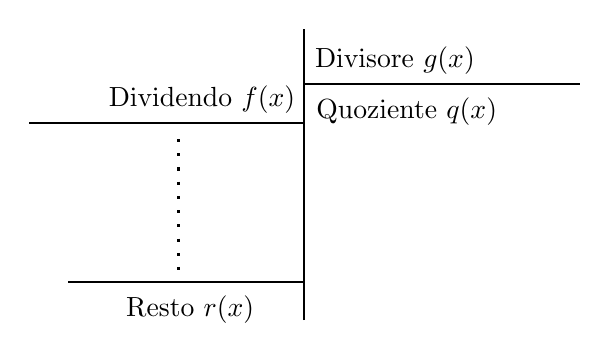
\begin{tikzpicture}
        \draw[thick] (0,0) -- (0,3.7);
        \draw[thick] (0,3) -- (3.5,3);
        \draw[thick] (0,2.5) -- (-3.5,2.5);
        \draw[thick] (0,0.48) -- (-3,0.48);
        \draw[line width=0.4mm, loosely dotted] (-1.6,2.3) -- (-1.6,0.6);

        \node at (1.15,3.3) {Divisore \(g(x)\)};
        \node at (-1.3,2.8) {Dividendo \(f(x)\)};
        \node at (1.3,2.65) {Quoziente \(q(x)\)};
        \node at (-1.45,0.13) {Resto \(r(x)\)};
    \end{tikzpicture}
\end{center}

\sexample{Divisione polinomi}{
    Prendiamo \(f(x)=4x^5+3x^3 + 2x^2 - x + 1\) e \(g(x)=2x^3 + 2\).\\
    Allora \(f(x) = g(x)(2x^2 + \frac{3}{2}) + (-2x^2 - x - 2)\)
}

\subsection{Equazioni algebriche}

\sdefinition{Equazione algebrica}{
    Un'equazione \textit{algebrica} è una equazione del tipo \(f(x)=0\)
    dove \(f(x)\) è un polinomio non-nullo.
}

Il grado di una equazione algebrica è il grado del polinomio.

\stheorem{Teorema del resto}{
    Dato un polinomio \(p(x)\) e un numero \(\alpha \in \mathbb{R}\),
    la divisione di \(p(x)\) per \(x- \alpha\) ha resto \(p(\alpha)\).
    \[
        p(x)=q(x)(x-\alpha) + p(\alpha)
    \]
}

\sproof{Teorema del resto}{
    Dividendo \(p(x)\) per \(x-\alpha\) troviamo che \(f(x)\) è uguale a
    \[
        p(x)=q(x)(x-\alpha) + r(x)
    \]
    dove \(r(x)=0\) oppure \(\deg r(x) < \deg x - \alpha = 1\).
    Quindi \(r(x)\) è costante.
    Abbiamo allora \(p(x)=(x-\alpha) q(x) + r(x)\) e quindi
    \[
        p(\alpha) = (\alpha - \alpha)q(x) + r(x) = r(x)
    \]
    e quindi \(r(x) = p(\alpha)\).
}

\scorollary{}{
    Il valore \(\alpha\) è soluzione di \(f(x)=0\) se e solo se
    \(f(x)=(x-\alpha)q(x)\) per qualche \(q(x)\).
}

\scorollary{Numero di soluzioni di equazione algebriche}{
    Se \(f(x)=0\) è un'equazione algebrica di grado \(n\),
    allora ha al massimo \(n\) soluzioni distinte.
}

\sproof{Numero di soluzioni di equazione algebriche}{
    Siano \(a_1\), \(a_2\), \(\cdots\), \(a_t\) soluzioni distinte di \(f(x)=0\)
    dove \(f(x)\) non è nullo.
    Dobbiamo dimostrare che \(t<n\).
    Per il teorema del resto \(f(x)=(x-a_1)q_1(x)\) per qualche polinomio \(q_1(x)\).
    Lo stesso vale per \(a_2\), \(a_3\), \(\cdots\).
    Sostituendo otteniamo quindi
    \(0=f(a_2)=(a_2-a_1)q_1(a_2)\).
    Poiché \(a_1 \neq a_2\), abbiamo allora (per il principio di annullamento)
    che \(q_1(a_2)=0\). Per il teorema del resto \(q_1(x)=(x-a_2)q_2(x)\) per qualche \(q_2(x)\),
    e quindi \(f(x) = (x-a_1)(x-a_2)q_2(x)\).
    Per induzione, giungiamo a \(f(x)=(x-a_1)(x-a_2)\cdots(x-a_t)q_t(x)\)
    e confrontando i gradi troviamo che \(t \leq n\).
}

\subsection{Soluzioni di equazioni polinomiali semplici}

L'equazione di primo grado \(ax+b=0\) con \(a\neq 0\)
ha un'unica soluzione data da \(x = -\frac{b}{2}\).

L'equazione di secondo grado \(ax^2 + bx + c = 0\) con \(a\neq 0\)
e \(\Delta = b^2 - 4ac\) ha
\begin{align*}
\begin{cases}
    0 & \Delta <0 \\
    1 & \Delta =0 \\
    2 & \Delta >0
\end{cases}
\end{align*}
soluzioni date da
\[
    x_{1,2} = \frac{b \pm \sqrt{\Delta}}{2a}
\]

A partire dalle equazioni di secondo grado, non esiste una formula risolutiva.

\sexample{}{
    La seguente equazione non è algebrica, in quando gli oggetti non sono polinomi, ma potremo
    ricondurla ad una tale equazione.
    \begin{align*}
        -\frac{x}{4-x^2} &= \frac{1}{x_2} - \frac{2}{x^2 + 4x + 4} \\
    \end{align*}
    Bisogna innanzitutto verificare per quali valori di \(x\) le funzioni coinvolte sono definite.
    In quando caso, quando il denominatore è diverso da zero.
    \[
        4-x^2 \neq 0 \land x-2 \neq 0 \land x^2 +4x+4 \neq 0
    \]
    per cui \(x \neq 2 \land x \neq -2\).
    \begin{align*}
        -\frac{x}{(2-x)(2+x)} &= \frac{1}{x-2} - \frac{2}{(x+2)^2}
    \end{align*}
    La moltiplicazione per \((2-x)(2+x)^2\) \textit{rischia} di introdurre le soluzioni \(x=2\) e \(x=-2\).
    \begin{align*}
        -x(2+x) &= -(2+x)^2 - 2(2-x) \\
        -2x - x^2 &= -4-4x-x^2-4+2x \\
        0 &= -8
    \end{align*}
    E quindi non abbiamo nessuna soluzione.
    Se ci fossero state delle soluzioni, avremmo dovuto scartare i valori \(2\) e \(-2\)
    per le condizioni di esistenza.
}

\pagebreak

\section{Disequazioni}

\sdefinition{Disequazione}{
    Una \textit{disequazione} è una funzione del tipo
    \(f(x)\neq g(x)\), \(f(x)>g(x)\) oppure \(f(x)\geq g(x)\)
    dove \(f(x)\) e \(g(x)\) sono funzioni reali.
}

Come si comportano le operazioni in \(\mathbb{R}\) rispetto all'ordinamento?
\sproposition{}{
    Dati \(a,b\in\mathbb{R}\) abbiamo
    \begin{align*}
        a \leq b &\iff a+c\leq b+c \\
        a \leq b &\iff ac\leq bc, \quad c > 0
    \end{align*}
}

\sexercise{}{
    \begin{align*}
        \frac{x}{x-2} \neq \frac{2}{2x-x^2} - \frac{3}{x}
    \end{align*}
    Le condizioni di esistenza sono \(x \neq 2 \land x \neq 0\).
    Risolviamo l'equazione associata
    \begin{align*}
        \frac{x}{x-2} = \frac{2}{2x-x^2} - \frac{3}{x}
    \end{align*}
    e troviamo le soluzioni \(x = 1\) e \(x=-4\).
    Per cui, le soluzioni della disequazione sono
    \[
        \{ x \,|\, x \neq 2 \land x \neq 0 \land x \neq 1 \land x \neq -4 \}
    \]
}

\sexercise{}{
    \begin{align*}
        \frac{x}{x-2} \leq \frac{2}{2x-x^2} - \frac{3}{x}
    \end{align*}
    In questo caso \textbf{non} è possibile moltiplicare per \(x(x-2)\) perché questo
    assume valori non sempre positivi.
    Si procede per
    \begin{align*}
        \frac{x}{x-2} - \frac{2}{2x-x^2} + \frac{3}{x} &\leq 0 \\
        \frac{x^2 + 2 + 3(x-2)}{x(x-2)} &\leq 0 \\
        \frac{x^2 + 3x - 4}{x(x-2)} &\leq 0 
    \end{align*}
    Sappiamo che \(x^2 + 3x - 4\) si annulla per \(x=1\) e \(x=-4\), e per il teorema del resto
    abbiamo che \(x^2 + 3x - 4 = (x-1)(x+4)\).
    \begin{align*}
        \frac{(x-1)(x+4)}{x(x-2)} \leq 0
    \end{align*}
    Dallo studio dei segni di \(x-1\), \(x+4\), \(x\) e \(x-2\)
    possiamo determinare il segno dell'intera funziona nei vari intervalli.
    Giungiamo quindi alla soluzione
    \[
        x \in [-4;0) \cup [1;2)
    \]
}

\pagebreak

\section{Potenze di numeri}

\subsection{Potenze di numeri reali con esponenti interi}

\sdefinition{Potenza intera su numero reale}{
    Dato \(a\in \mathbb{R}\) e \(n\in\mathbb{N}\),
    il valore \(a^n\) viene definito con la seguente ricorrenza:
    \[
        a^n = \begin{cases}
            1 & n=0 \\
            a^{n-1} & n > 0 \\
            \frac{1}{a^n} & < 0
        \end{cases}
    \]
    per \(a \neq 0 \land n \neq 0\).
}

È convenzionalmente possibile anche definire \(0^0=1\).
Mediante queste definizioni è possibile dimostrare per induzione
le seguenti proprietà:

\sproposition{Proprietà potenze}{
    Dato \(a,b\in \mathbb{R}\) e \(n,m\in{\mathbb{N}}^+\),
    \begin{enumerate}
        \item \(a^na^m = a^{m+n}\)
        \item \({(a^m)}^n = a^{mn}\)
        \item \((ab)^n = a^n b^n\)
    \end{enumerate}
}

\subsection{Radicali}

\sproposition{Esistenza radicale}{
    Dato \(\alpha\in{\mathbb{R}}^+\) e \(n\in{\mathbb{N}}^+\),
    esiste un unico \(\beta\in{\mathbb{R}}^+\) tale che
    \[
        \beta^n = \alpha
    \]
    Nel caso \(n\) sia pari, \({(-\beta)}^n = a\).
}

Se \(n\) è pari, i valori per beta possono essere due.

\sdefinition{Radicale}{
    Dato \(\alpha\in\mathbb{R}\) e \(n\in{\mathbb{N}}^+\),
    il valore positivo \(\beta\) tale che \(\beta^n = \alpha\) viene denotato \(\sqrt[n]{\alpha}\). 
    Questo valore è definito per
    \[
        \begin{cases}
            \sqrt[n]{\alpha} \geq 0 & n \text{ pari} \\
            \sqrt[n]{\alpha} \in \mathbb{R} & n \text{ dispari} \\
        \end{cases}
    \]
}

\sproposition{Proprietà dei radicali}{
    Dato \(\alpha\in\mathbb{R}\) e \(n,m\in{\mathbb{N}}^+\),
    \[
        \sqrt[m]{\sqrt[n]{\alpha}} = \sqrt[mn]{\alpha}
    \]
    qualunche siano \(m,n\) se \(\alpha \geq 0\), mentre solo se \(m\) e \(n\)
    sono entrambi dispari se \(\alpha < 0\).
}

\pagebreak

\sdefinition{Valore assoluto}{
    Dato \(\alpha \in \mathbb{R}\),
    il \textit{valore assoluto} è dato da
    \[
        |\alpha| = \begin{cases}
            \alpha & \alpha \geq 0 \\
            -\alpha & \alpha < 0
        \end{cases}
    \]
}

\sproposition{Radicale di quadrato}{
    Dato \(\alpha\in\mathbb{R}\),
    \[
        \sqrt{{\alpha}^2} = |\alpha|
    \]
}

\sproposition{Semplificazione dei radicali}{
    Dato \(\alpha\in\mathbb{R}\) e \(n,m,k\in{\mathbb{N}}^+\),
    l'espressione
    \[
        \sqrt[kn]{{\alpha}^{km}} =
        \begin{cases}
            \sqrt[n]{{|\alpha|}^m} & k \text{ pari} \\
            \sqrt[n]{{\alpha}^m} & k \text{ dispari} \\
        \end{cases}
    \]   
}

\subsection{Potenze di numeri reali con esponenti razionali positivi}

\sdefinition{Potenza razionale positiva su numero reale}{
    Dato \(a\in {\mathbb{R}}^+\) e \(q\in\mathbb{Q}\)
    con \(q = \frac{m}{n}\) dove \(m, n \in {\mathbb{N}}^+\),
    il valore \(a^q\) viene definito nella seguente maniera:
    \[
        a^q = \sqrt[n]{a^m}
    \]
    per \(a \neq 0 \land q \neq 0\).
}

Il motivo per cui la potenza razionale non è definita per una base negativa
in quando il valore cambia se la frazione dell'esponenze viene espressa in un altro modo.
Per esempio \({(-2)}^{\frac{1}{3}} \neq {(-2)}^{\frac{2}{6}}\).
Considerando solo gli esponenti ridotti ai minimi termini, cadrebbero le proprietà delle potenze.

\sexercise{Radicali}{
    \begin{align*}
        \frac{\sqrt[3]{a^3 + a^4}}{\sqrt{a}} \cdot
        {\left(
            \sqrt[4]{\frac{1+a}{a}} + \frac{a \sqrt[12]{1+a}}{\sqrt[4]{a}}
        \right)}^{-1}
    \end{align*}
    Gli argomenti di radicali con esponenti dispari, non danno problemi.
    Gli argomenti di radicali con esponenti pari, devono essere non negativi.
    Dunque abbiamo queste condizioni
    \[ a \geq 0 \land \frac{1+a}{a} \geq 0 \land 1 + a \geq 0 \]
    Inoltre, i divisori devono essere diversi da \(0\).
    \[ \sqrt{a} \neq 0 \land a \neq 0 \land \sqrt[4]{\frac{1+a}{a}} \neq 0 \land \sqrt[4]{a} \neq 0 \]
    Le prime condizioni possono essere semplificate a
    \( a \geq 0 \)
    Le seconde condizioni assieme alle prime possono essere ricondotte a \(a > 0\).
    Semplificando l'espressione otteniamo
    \[
        2 \sqrt[4]{a^3}\sqrt[12]{1+a}
    \]
}

% sqrt[3]{x(x^2 - 2)} = x+2
% sqrt{x^2-x-6} = sqrt{3x-x^2} sol=3


% sqrt{x^2-x-6} > sqrt{3x-x^2}
% Le condizioni iniziali sono le medesime dell'equazione precedente
% Sotto le condizioni iniziali posso elevare al quadrato perché se a  b >= 0, allora a^2 >= b^2 >= 0
% Si ottiene la disequazione
% x^2 - x - 6 > 3x - x^2
% Abbiamo dunque il sistema:
% 1) x^2 - x - 6 >= 0
% 2) 3x - x^2
% 3) x^2 - x - 6 > 3x-x^2
% Tuttavia, una è ridondante e possiamo semplificare il sistema 
% La seconda e la terza implicano la prima.
% È sufficiente risolvere il sistema 3x-x^2 >= 0 \land x^2 - x - 3 > 3x - x^2
% Semplificando otteniamo il sistema
% 1) 3x - x^2 >= 0
% 2) x^2 - 2x - 3 > 0
% Dalla tabella dei segni otteniamo

\subsection{Potenze di numeri reali con esponenti reali}

\textbf{Proprietà dei numeri reali}
Siano \(A\) e \(B\) due insiemi non vuoti di numeri reali
tale che:
\begin{itemize}
    \item per ogni \(x\in A\) e ogni \(y \in B\), si ha \(x < y\).
    \item oer ogni \(k > 0\) esiste \(x \in A\) e \(y \in B\) tale che
        \(d(x,y) < k\), cioè \(y-x < k\).
\end{itemize}
Allora, esiste un unico numero reale tale che \(x \leq r \leq y\)
per ogni \(x \in A\) e \(y \in B\).

\sdefinition{Potenza reale su numero reale}{
    Dato un numero \(\alpha \in \mathbb{R}\) e \(r\in \mathbb{R}\).
    Per caso il caso \(\alpha > 1 \).
    Si può dimostrare che se \(p < q\) sono due razionali, allora \(\alpha^p < \alpha^q\).
    Allora, considerando i due insiemi
    \[
        A = \{ \alpha^p \,|\, p \in \mathbb{Q}, p < r \}
    \]
    e
    \[
        B = \{ \alpha^q \,|\, q \in \mathbb{Q}, q < r \}
    \]
    ogni elemento di \(A\) è minore di ogni elemento di \(B\).
    Inoltre, si può dimostrare che \(A\) e \(B\) sono due insiemi
    che soddisfano anche la seconda richiesta proprietà di prima, cioè la vicinanza arbitraria.
    Dunque, esiste un unico reale \(s\) tale che \(x \leq s \leq y\) per ogni
    \(x\in A\) e ogni \(y \in B\).
    Poniamo allora
    \[
        \alpha^r = s
    \]
    La definizione oer \(\alpha = 1\) è data data \(\alpha^r = 1\). \\
    La definizione per \(\alpha < 1\) è analoga (con ordinamento scambiato).
}

La definizione è ben posta e si può dimostrare che in questo modo le prorpietà delle potenze si estendono.

\sproposition{Proprietà potenze reali}{
    \[
        a^r a^s = a^{r+s}, \quad a>0 \land r,s\in\mathbb{R}
    \]
    \[
        {(a^r)}^s = a^{rs}, \quad a>0 \land r,s\in\mathbb{R}
    \]
    \[
        (ab)^r = a^r b ^r, \quad a,b\geq0
    \]
    Inoltre,
    \[
        a^r < a^s \iff a>1 \land r<s
    \]
    \[
        a^r > a^s \iff 0<a<1 \land r<s
    \]
}

%%% grafico della funzione esponenziali, cioè della funzione che manda un numero reale \(r\)
%%% in \(a^r\) con a reale positivo fissato.

%Se \(a > 1\)
%\begin{tikzpicture}[
%    scale=2,
%    declare function={
%        func(\x) = 2^\x;
%        Width=3;
%        Height=2;
%    }
%]
%    \draw[domain=-0.5:3, smooth, variable=\x, blue, very thick] plot ({\x}, {func(\x)});
%    
%    \draw[->] (0, -0.25) -- (0, Height) node[right] {\(y\)};
%    \draw[->] (-0.25, 0) -- (Width, 0) node[above] {\(x\)};
%\end{tikzpicture}
%
%Se \(0 < a < 1\)
%
%\begin{tikzpicture}[
%    scale=2,
%    declare function={
%        func(\x) = 0.25^\x;
%        Width=3;
%        Height=2;
%    }
%]
%    \draw[domain=-0.5:3, smooth, variable=\x, blue, very thick] plot ({\x}, {func(\x)});
%    
%    \draw[->] (0, -0.25) -- (0, Height) node[right] {\(y\)};
%    \draw[->] (-0.25, 0) -- (Width, 0) node[above] {\(x\)};
%\end{tikzpicture}
%
% Se a=1

Tra gli esponenziali, di particolare importanza, è quello di base numero di Eulero \(e\),
un numero definito per procedimento di limite.

\pagebreak

\section{Disequazioni son valore assoluto}

Supponiamo di avere una disequazione \(k \geq |g(x)|\)
con \(k \geq 0\), allora \(-k \leq g(x) \leq k\).
Nel caso in cui \(k <0\), la disequazione non avrebbe soluzioni.

Se, al posto di \(k\), avessimo una funzione, come in
\[ f(x) \geq |g(x)| \]
si potrebbe comunque studiare il segno di \(f(x)\)
per verificre quando è positivo.
Tuttavia, ciò non è strettamente necessario.
Possiamo considerare il valore assoluto come \(|a| = \max{a, -a}\).
Allora, \(f(x) \geq |g(x)|\) è equivalente a \(f(x) \geq \max {g(x), -g(x)} \)
e quindi \(-f(x) \leq g(x) \leq f(x)\).
Analogamente, lo stesso ragionamento vale per \(f(x) \leq |g(x)\),
il che è equivalente a \(g(x) \leq -f(x) \lor g(x) \geq f(x)\).

% \sqrt{x^2 - |2x+1|} > x-1
% se x-1 < 0, la disequazione è soddisfatta (pur soddisfando le condizioni iniziali)
%            2x-1 > |2x+1|
%            Potrei trattare questa disequazione come prima ma noto che sto ipotizzando che x-1 >= 0
%            e, dunque, 2x+1>=0, cioè |2x+1|=2x+1
%            la cui equazione diventa 2x-1 > 2x + 1 che non ha soluzioni
%            le soluzioni sono date allora da x-1 <0 AND x² - 2x - 1 >= 0 AND x² + 2x + 1 >= 0
%            1) x < 1
%            2) x <= 1-sqrt(2) OR x >= 1+sqrt(2)
%            3) la terza è sempre soddisfatta
% Abbiamo allora l'unione di tutte e 3: x <= 1-sqrt(2)

% ============ Altro esercizio
% sqrt{x^2 - x - 6} \leq sqrt{5x - 2x^2}
% Risolviamo l'equazione associata.
% Condizioni iniziali x^2 - x-6 >= 0 AND 5x - 2x^2 >= 0
% Nell'ipotesi che le condizioni inizuali siano soddisfatte eleviamo al quadrato e troviamo
% x^2 - x - 6 = 5x - 2x^2 cioè
% 3x^2 - 6x - 6 che ha soluzioni x_1,2 = 1 +- sqrt{3}
% Verifico le condizioni ma entrambe non funzionano, quindi non ci sono soluzioni
% Ora per la disequazione (stesse condizioni iniziali), elevo al quadrato.
% Elevo al quadrato e trovo x^2 - x - 6 >= 5x - 2x^2 AND x^2 - x - 6 >= 0 AND 5x-2x^3 >= 0
% La prima e la terza implicano la seconda, quindi può essere rimossa
% cioè 3x^2 - 6x - 6 >= 0 AND -2x^2 + 5x >= 0
% => 

\section{Logaritmi}

L'esponenziale è definiti per basi \(a > 0\).
Assume, al variare di \(x\), tutti i valori reali positivi se \(x \neq 1\).

\sdefinition{Logaritmi}{
    La soluzione dell'equazione
    \[ a^x = b \]
    con \(b >0\) e \(a > 0 \land a \neq 1\),
    è pari al \textit{logaritmo}
    di \(b\) in base \(a\)
    \[
        x = \log_a(b)
    \]
}

Le proprietà dei logaritmi sono analoghe a quelle dell'espnonenziale.
\sproposition{Proprietà dei logaritmi} {
    \[
        \log_a(xy) = \log_a(x) + \log_a(y)
    \]
    \[
        \log_a(x^y) = y\log_a(x)
    \]
    \[
        \log_a(b) = \frac{\log_c(a)}{\log_c(b)}
    \]
}

% Come trovatre la terza


Il passaggio da moltiplicazione e somma di logaritmi, potrebbe non avere senso
nella seconda forma.
E.g \(\ln(x(x-1))\) non is può riscrivere come \(\ln(x) + \ln(x-1)\)
perché, se sono positivi quando moltiplicati, non è detto che lo siano separatamente.

Se abbiamo \(\log_2(x^2)\), possiamo riscriverlo come \(2 \log_2|x|\).

%%% Esercizi

\sexercise{Logaritmi}{
    \(\log_2(x) + \log_3(x-1)\) è definito per \(x > 1\).
    Per portare tutto in base \(2\) è necessario
    eseguire la seguente operazione 
    \begin{align*}
        \log_2x + \log_32\cdot\log_2(x-1) &= log_2x + {\log_2(x-1)}^{\log_3(2)} \\
        &= \log_2(x{(x-1)}^{\log_3(2)})
    \end{align*}
}

\sexercise{}{
    L'equazione
    \[ 3^{x+1} = 5 \]
    ha soluzione \(x = 1 \log_3(5)\).
}

\sexercise{}{
    L'equazione
    \[ \log(x-1) + \log(2x+1) = 2\log(x+1) \]
    ha condizioni iniziali \(x > 1\).
    \begin{align*}
        \log(x-2)(2x-1) &= \log{(x+1)}^2 \\
        &= (x-1)(2x-1) = {(x+1)}^2 \\
        &= x^2 -5x = 0
    \end{align*}
    che ha come soluzioni \(x=0\) e \(x=5\).
    Di queste solo \(x=5\) è compatibile con la condizione di esistenza.
}

\pagebreak

\section{Sistemi lineari}

\sdefinition{Sistema lineare}{
    Un \textit{sistema lineare} di \(m\) equazioni in \(n\) incognite è un sistema del tipo
    \[
        \begin{cases}
            a_{1,1}x_1 + a_{1,2}x_2 + \cdots + a_{1,n}x_n = b_1 \\
            a_{2,1}x_1 + a_{2,2}x_2 + \cdots + a_{2,n}x_n = b_2 \\
            \cdots \\
            a_{m,1}x_1 + a_{m,2}x_2 + \cdots + a_{m,n}x_n = b_m
        \end{cases}
    \]
    dove \(a_{i,j} \in \mathbb{R}\) e \(x_j\) sono incognite.
}

Le soluzioni di un tale sistema sono n-uple.

\sexample{Sistema equazioni}{
    \[
        \begin{cases}
            2x - 3y + \sqrt{3} - 7w = 2 \\
            x +0y + 4z - 11w = 1
        \end{cases}
    \]
    In questo caso le soluzioni sono quaterne.
}

\sexample{Sistema equazioni}{
    Un sistema lineare con forma
    \[
        \begin{cases}
            3x = z \\
            5y = -7 \\
            3z = 4\pi
        \end{cases}
    \]
    ha un'unica soluzione \((x,y,z) = (\frac{2}{3}, -\frac{7}{5}, \frac{4\pi}{3})\).
}

\sexample{Sistema equazioni}{
    Un sistema lineare con forma
    \[
        \begin{cases}
            3x + 5w = 2 \\
            2y = \sqrt{5} \\
            3z - 2w = \sqrt[3]{3}
        \end{cases}
    \]
    si può risolvere trattando \(w\) come un parametro, e trovare le soluzioni accordatamente.
    La soluzione è \((x,y,z,w) = (\frac{2-5w}{3}, \frac{\sqrt{5}}{2}, \frac{\sqrt[3]{3}-2w}{3}, w)\),
    ossia un insieme infinito di soluzioni, in funzione di \(w\) (parametro libero).
}

Le trasformazioni lecite su un sitema sono quelle reversibili:
\begin{itemize}
    \item riordinare l'ordine delle equazioni;
    \item moltiplicare un'equazione per una costante non nulla;
    \item sostituire a un'equazione la somma tra quella equazione e \(k\) volte un'altra.
\end{itemize}

\pagebreak

\sexample{Trasformazioni sistemi lineari}{
    \[
        \begin{cases}
            3x + 2y + 5z + 7w = 2 \\
            2x - 3z - w = 5 \\
            6y - z = 3w = 2
        \end{cases}
    \]
    È possibilare sommare alla seconda equazione \(3\) volte la prima, si trova
    \[
        \begin{cases}
            3x + 2y + 5z + 7w = 2 \\
            11x + 6y - 12z + 20w = 11 \\
            6y - z = 3w = 2
        \end{cases}
    \]
    In questo modo ho ottenuto un altro sistema equivalente ma non mi sono avvicinato alla soluzione.
    Avrei potuto generalmente sommare alla seconda equazione \(k\) volte la prima, e notare che
    con \(k=-\frac{2}{3}\) si ottiene del progresso.
    \[
        \begin{cases}
            3x + 2y + 5z + 7w = 2 \\
            0x - \frac{4}{3}y - \frac{14}{3}z - \frac{17}{3}w = \frac{11}{3} \\
            6y - z = 3w = 2
        \end{cases}
    \]
    Così facendo, nella terza equazione l'incognita \(x\) non compare.
    Adesso, è possibilire usare la seconda equazione per eliminare la \(y\) dalla terza equazione.
    \[
        \begin{cases}
            3x + 2y + 5z + 7w = 2 \\
            -\frac{4}{3} y - \frac{19}{3} z - \frac{17}{3}w = \frac{11}{3} \\
            \frac{59}{2}z - \frac{45}{2} w = \frac{35}{2}
        \end{cases}
    \]
    Trattando \(w\) come un parametro libero, dall'ultima equazione calcoliamo
    \(z\) in funzione di \(w\), dalla seconda calcolo \(y\) in funzione di \(z\)
    e infine \(x\) in funzione di \(w\).
}

\sexample{}{
    \[
        \begin{cases}
            3y-2z-5w = 1 \\
            x - y + z + 3w = 2 \\
            2x + y - w = 3 \\
            3x + 2y + 3z - 3w = 0
        \end{cases}
    \]
    Non è possibile utilizzare la prima equazione per eliminare la \(x\),
    ma è possibile utilizzare la seconda per eliminarla dalle altre.
    Sottraiamo quindi 2 volte la seconda dalla terza, 3 volte la seconda dalla quarta.
    \[
        \begin{cases}
            3y-2z-5w = 1 \\
            x - y + z + 3w = 2 \\
            3y - 2z -7w = -1 \\
            5y - 12w = -6
        \end{cases}
    \]
}

Vi è il rischio che un'incognita eliminata venga reintrodotta quando si prova ad eliminarne una seconda.
Per evitare il problema, dopo aver utilizzato una equazione una certa equazione per eliminare una certa incognita,
è cosa furba portare tale equazione in testa al sistema, e successivamente continuo
lavorando sulle successive.

\sexercise{Sistema senza soluzioni}{
    \[
        \begin{cases}
            2x + 2y + 5z = 1 \\
            2x - 3y + 4z = 4 \\
            7y - 4y + 13z = 6
        \end{cases}
    \]
    Usiamo la prima equazione per eliminare la \(x\) dalle successive
    \[
        \begin{cases}
            3x + 2y + tz = 1 \\
            -\frac{13}{5}y + \frac{2}{3}z = \frac{10}{3} \\
            \frac{26}{3}y + \frac{4}{3}z = \frac{11}{3}
        \end{cases}
    \]
    Usiamo la seconda equazione per eliminare la \(y\) dalla successiva.
    \[
        \begin{cases}
            3x + 2y + tz = 1 \\
            -\frac{13}{5}y + \frac{2}{3}z = \frac{10}{3} \\
            0 = -3
        \end{cases}
    \]
    Di conseguenza, il sistema \textit{non} ha soluzioni in quanto l'ultima equazione non è mai soffisdatta.
}

Nel caso ottenessimo un'equazione del tipo \(0x + 0y + 0z + \cdots = 0\), ossia un'identità,
essa può essere scartata in quanto non contiene nessuna infromazione necessaria.

\pagebreak

\section{Trigonometria}

Per introdurre le funzioni goniometrica è comodo impostare come sistema di riferimento
il piano cartesiano:
\begin{itemize}
    \item un punto fissato \(O\), detto \textit{origina};
    \item due rette ortogonali tra loro e passanti per \(O\), dette \textit{assi};
    \item due punti \(U_1\) e \(U_2\), sugli stessi assi, posti alla stessa distanza non nulla da \(O\),
    detti \textit{punti unitari}.
\end{itemize}


\DeclareRobustCommand{\widefrac}[3][5pt]{%
  \frac{\hspace{#1}#2\hspace{#1}}{\hspace{#1}#3\hspace{#1}}}

Fatto ciò, posso assegnare ad ogni punto \(P\) del piano una coppia di reali \(x_p, y_p\)
detti \textit{coordinate} del punto \(P\).
Per trovare \(x_p\) considero la proiezione ortogonale di \(x\) sull'asse che contiene \(U_1\),
trovando un certo punto \(H\). Si considera il rapporto tra le lunghezze del segmento \(\overline{OH}\)
e la lunghezza del segmento \(\overline{OU_1}\). Poniamo poi
\[
    x_p = \begin{cases}
        \widefrac{\overline{OH}}{\overline{OU_1}} & \text{ se } H \text{ e } U_1 \text{ stanno sulla stessa semiretta di origine } O \\
        -\widefrac{\overline{OH}}{\overline{OU_1}} & \text{ altrimenti}
    \end{cases}
\]
Analogamente, per \(x_p\)
\begin{itemize}
    \item la retta \(OU_1\) è detta \text{asse delle x} o \text{asse delle ascisse};
    \item la retta \(OU_2\) è detta \text{asse delle y} o \text{asse delle ordinate};
\end{itemize}

Se \(P\) e \(Q\) sono due punti diversi, almeno una delle due proiezioni e quindi \(P\)
e \(Q\) hanno almeno una coordinata diversa; in altri termini la coppia \((x_p, y_p)\)
individua \(P\). Viceversa, data una coppia di numeri reali \((x,y)\) si trova
un unico punto che ha esattamente \((x,y)\) come coordinate.
Dunque, possiamo identificare il piano con l'insieme delle coppie ordinate dei numeri reali \({\mathbb{R}}^2\).

(In realtà, non è strettamente necessario considerare tutte le coppie di numeri reali
per soddisfare gli assiomi euclidei)

Supponiamo di avere una semiretta \(s\) uscente dall'origine.
È possibile associare un angolo \(\theta\) fra la semiretta e l'ascisse.
Chiaramente, lo stesso angolo può assumere anche i valori \(\theta +2k\pi\) \(k\in\mathbb{N}\) oppure,
l'angolo inverso, \(2\pi-\theta\). Quindi, abbiamo infiniti angoli che quantificano la stessa
ampiezza di semiretta.

Questo sistema, detto \textit{radiante}
prende come riferimento il valore \(2\pi\) per quantificare un giro completo attorno all'origine.
Una semiretta con ampiezza 1 radiante, forma un arco di lunghezza dell'arco stesso.

Esiste anche il sistema sessagesimale dove un angolo giro equivale a \(360^\circ\).
La conversione da radianti \(x\) e \(x^\circ\) è data da
\[
    x^\circ = \frac{180^\circ}{\pi}
\]

\sdefinition{Funzione seno}{
    Dato un angolo \(\theta\), la circonferenza di raggio \(1\) centrata nell'origine e
    una semiretta di lunghezza \(1\) che si estende dall'origine alla circonferenza con
    ampiezza \(\theta\). Consideriamo il punto \(P\) come il punto di intersezione fra la semiretta
    e la circonferenza.
    Il valore \(\sin \theta\) rappresenta la distanza fra l'origine e il punto
    della proiezione di \(P\) sulle ascisse.
}

\sdefinition{Funzione coseno}{
    Dato un angolo \(\theta\), la circonferenza di raggio \(1\) centrata nell'origine e
    una semiretta di lunghezza \(1\) che si estende dall'origine alla circonferenza con
    ampiezza \(\theta\). Consideriamo il punto \(P\) come il punto di intersezione fra la semiretta
    e la circonferenza.
    Il valore \(\cos \theta\) rappresenta la distanza fra l'origine e il punto
    della proiezione di \(P\) sulle ordinate.
}

\pagebreak

\sdefinition{Funzione tangente}{
    Dato un angolo \(\theta\), la \textit{tangente}
    è definita come
    \[
        \tan\theta = \frac{\sin\theta}{\cos\theta}
    \]
    quando \(\cos\theta \neq 0\).
}

Il coseno è pari a zero solo quando \(\theta = \frac{\pi}{2} + k\pi\) per \(k\in\mathbb{N}\).

\begin{center}
    \begin{tikzpicture}[scale=3.75]
        \definecolor{darkgreen}{rgb}{0.0, 0.7, 0.0}
        % Draw the x and y axes
        \draw[thick, ->] (-1.5,0) -- (1.5,0) node[right] {$x$};
        \draw[thick, ->] (0,-1.5) -- (0,1.5) node[above] {$y$};
    
        % Draw the unit circle
        \draw (0,0) circle (1);
    
        % Draw the angle theta
        \draw[thick, blue] (0,0) -- (0.866,0.5) node[right] {$P(x,y)$};
        \draw[dashed, blue] (0,0) -- (0.866,-0.5) node[right] {\ $P'(x,-y)$};
    
        % Draw dashed lines to indicate the projections on the axes
        \draw[dashed] (0.866,-0.5) -- (0.866,0.5) -- (0,0.5);
    
        % Label the angle theta
        \draw (0.3,0) arc (0:30:0.3);
        \node at (0.35,0.10) {$\theta$};
    
        % Label the origin
        \node at (-0.06, -0.06) {$O$};
    
        % Draw the projections on the axes
        \draw[thick, red] (0,0) -- (0.866, 0) node[midway, below] {$\cos \theta$};
        \draw[thick, darkgreen] (0.866,0) -- (0.866, 0.5) node[midway, left] {$\sin \theta$};
    
        % Additional labels and lines
        %\node at (-1.075, 0.05) {-1};
        \node at (-0.1, 1.1) {\(U_2\)};
        \node at (1.075, 0.05) {\(U_1\)};
        %\node at (-0.05, -1.1) {\(U_2\)};
    
        % Labels for each quadrant
        \node at (1, 1) {I};
        \node at (-1, 1) {II};
        \node at (-1, -1) {III};
        \node at (1, -1) {IV};

        %others
        \draw (0.866,0) rectangle (0.816,0.05);
    \end{tikzpicture}
\end{center}

Notiamo che il punto \(P\), che sta sulla circonferenza, dista \(1\) dall'origine,
e forma un triangolo rettangolo in \((0, P_y)\).
Per il teorema di pitagora, abbiamo allora la seguente proposizione:

\sproposition{Relazione pitagorica}{
    Dato un \(\theta\in\mathbb{R}\),
    \[
        \sin^2\theta + \cos^2\theta = 1
    \]
}


\end{document}